\section{Programmeertalen}

\begin{frame}
  \frametitle{Programmeertalen}
  \begin{center}
    \begin{tikzpicture}
      \node[language] at (5,1) {Java};
      \node[language] at (2,3) {Javascript};
      \node[language] at (1,2) {\csharp};
      \node[language] at (-2,-1) {\cpp};
      \node[language] at (-4,2) {C};
      \node[language] at (0,-1) {Python};
      \node[language] at (1,4) {Ruby};
      \node[language] at (-2,3) {Rust};
      \node[language] at (-4,-2) {Coq};
      \node[language] at (3,-1) {TypeScript};
      \node[language] at (3,-2) {Flow};
      \node[language] at (4,0) {Erlang};
      \node[language] at (-1,1) {Scala};
      \node[language] at (-1,-2) {Clojure};
      \node[language] at (-3,0) {Haskell};
      \node[language] at (2,1) {Dart};
      \node[language] at (4,4) {Common Lisp};
      \node[language] at (-4,4) {Brainfuck};
      \node[language] at (0,0) {Visual Basic};
    \end{tikzpicture}
  \end{center}
\end{frame}

\begin{frame}
  \frametitle{Programmeertalen}
  \begin{itemize}
    \item Veel programmeertalen (duizenden)
    \item Waarom bestaan ze?
    \item Hoe verschillen ze van elkaar?
    \item Is het nuttig om er meerdere te kennen?
    \item Welke zien we in de opleiding?
  \end{itemize}
\end{frame}

\subsection{Wat is Programmeren?}

\begin{frame}
  \tableofcontents[currentsubsection]
\end{frame}

\begin{frame}
  \frametitle{Wat is Programmeren?}
  \begin{center}
    Programmeren is \\
    machine vertellen hoe reageren op inputs
  \end{center}
  \vskip5mm
  \begin{center}
    \begin{tikzpicture}[box/.style={minimum width=3cm,minimum height=1cm,draw,fill=blue!50,drop shadow},scale=0.8,transform shape]
      \node[box] (pc) {Computer};
      \node[box] (mouse) at (150:5) {Muis};
      \node[box] (keyboard) at (210:5) {Toetsenbord};
      \node[box] (screen) at (30:5) {Scherm};
      \node[box] (speakers) at (-30:5) {Speakers};

      \only<2-3>{
        \draw[-latex] (keyboard) -- (pc) node[below,midway,sloped,font=\tiny] {S ingedrukt};

        \only<3>{
          \draw[-latex] (pc) -- (screen) node[below,midway,sloped,font=\tiny] {toon S};
        }
      }

      \only<4-5>{
        \draw[-latex] (mouse) -- (pc) node[below,midway,sloped,font=\tiny] {klik op knop};

        \only<5>{
          \draw[-latex] (pc) -- (speakers) node[below,midway,sloped,font=\tiny] {klikgeluid};
          \draw[-latex] (pc) -- (screen) node[below,midway,sloped,font=\tiny] {toon ingedrukte knop};
        }
      }
    \end{tikzpicture}
  \end{center}
\end{frame}

\subsection{Waarom Bestaan Programmeertalen?}

\begin{frame}
  \tableofcontents[currentsubsection]
\end{frame}

\begin{frame}
  \frametitle{Waarom Bestaan Programmeertalen?}
  \begin{center}
    Time flies like an arrow \\
    Fruit flies like a banana \\[4mm]
    Plus de pain! \\[4mm]
    Veel diarree\kern1pt gevallen in Nickerie
  \end{center}
\end{frame}

\begin{frame}
  \frametitle{Waarom Bestaan Programmeertalen?}
  \begin{itemize}
    \item Spreektalen zijn vaak dubbelzinnig
    \item We kiezen onbewust voor de meest logische interpretatie
    \item Machines hebben geen ``common sense''
    \item Machine moet \emph{exacte} instructies ontvangen
    \item Programmeertalen zijn veel strikter en nauwkeuriger
  \end{itemize}
\end{frame}

\subsection{Hoe Werkt Programmeren?}

\begin{frame}
  \tableofcontents[currentsubsection]
\end{frame}

\begin{frame}
  \frametitle{Hoe Werkt Programmeren?}
  \begin{itemize}
    \item Taal biedt basisbouwblokken
    \item Taal biedt mogelijkheid om bouwblokken te combineren
    \item Zo ontstaan nieuwe bouwblokken (\emph{abstracties})
  \end{itemize}
\end{frame}

\begin{frame}
  \frametitle{Voorbeeld}
  \begin{center}
    \begin{tikzpicture}
      \draw (-5,-3) rectangle (5,3);
      \only<1>{
        \node {\ttfamily 0};
      }
      \only<2>{
        \node {\ttfamily 11001011};
      }
      \only<3>{
        \node[draw] {\ttfamily
          \begin{tabular}{c}
            10010101 \\
            10100110 \\
            01001010 \\
          \end{tabular}
        };
      }
      \only<4>{
        \begin{scope}[scale=0.4,transform shape]
          \foreach \x in {-10,-8,...,10} {
            \foreach \y in {-6,-4.5,...,6} {
              \node[draw,inner sep=2pt,font=\small] at (\x,\y) {\ttfamily%
                \tikzmath{
                  int \a;
                  int \b;
                  int \c;
                  \a = random(255);
                  \b = random(255);
                  \c = random(255);
                }%
                \parbox{1.5cm}{\centering%
                  {\setcounter{dummy}{\a}\padzeroes[8]{\binary{dummy}}} \\
                  {\setcounter{dummy}{\b}\padzeroes[8]{\binary{dummy}}} \\
                  {\setcounter{dummy}{\c}\padzeroes[8]{\binary{dummy}}}
                }
              };
            }
          }
        \end{scope}
      }
    \end{tikzpicture}
  \end{center}
  \begin{overprint}
    \onslide<1>
    \begin{center}
      Bit als eenvoudigste bouwblok
    \end{center}

    \onslide<2>
    \begin{center}
      Met 8 bits bouwen we een getal
    \end{center}

    \onslide<3>
    \begin{center}
      Drie getallen vormen samen een kleur
    \end{center}

    \onslide<4>
    \begin{center}
      Een tabel kleuren vormt een beeld
    \end{center}
  \end{overprint}
\end{frame}

\begin{frame}
  \frametitle{Abstractietoren}
  \begin{center}
    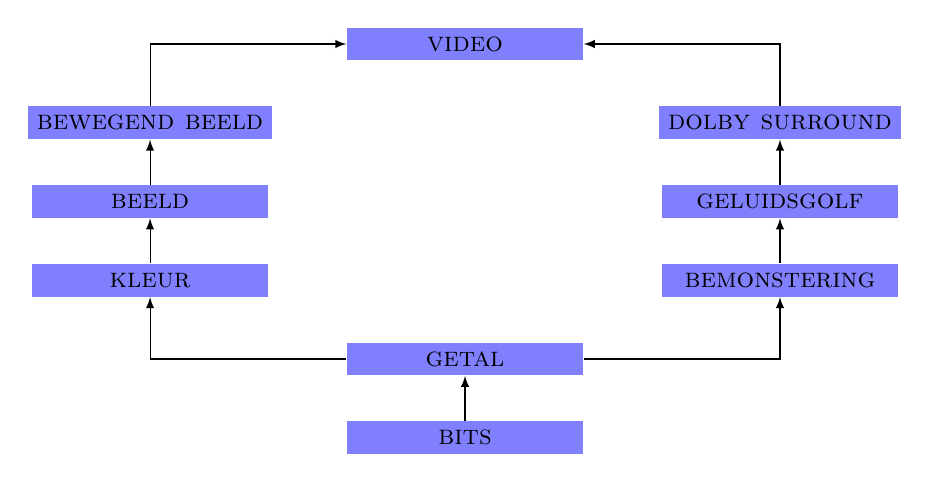
\begin{tikzpicture}[level/.style={fill=blue!50,minimum width=3cm,font=\scshape},
                        link/.style={-latex}]
      \node[level] (bits) at (0,0) {bits};
      \node[level] (number) at (0,1) {getal};
      \node[level] (color) at (-4,2) {kleur};
      \node[level] (image) at (-4,3) {beeld};
      \node[level] (animation) at (-4,4) {bewegend beeld};
      \draw[link] (bits) -- (number);
      \draw[link] (number) -| (color);
      \draw[link] (color) -- (image);
      \draw[link] (image) -- (animation);

      \node[level] (sample) at (4,2) {bemonstering};
      \node[level] (wave) at (4,3) {geluidsgolf};
      \node[level] (sound) at (4,4) {dolby surround};

      \draw[link] (number) -| (sample);
      \draw[link] (sample) -- (wave);
      \draw[link] (wave) -- (sound);

      \node[level] (movie) at (0,5) {video};
      \draw[link] (animation) |- (movie);
      \draw[link] (sound) |- (movie);
    \end{tikzpicture}
  \end{center}
\end{frame}

\subsection{Machinetaal}

\begin{frame}
  \tableofcontents[currentsubsection]
\end{frame}

\begin{frame}
  \frametitle{Moedertaal Machine}
  \begin{itemize}
    \item Verstaat de machine dan zoveel talen? \\[2mm]
    \item Zijn talen misschien machine-afhankelijk?
          \begin{itemize}
            \item Werkt Java enkel op Mac?
            \item Werkt Python enkel op Playstations?
          \end{itemize}
  \end{itemize}
\end{frame}

\begin{frame}
  \frametitle{Moedertaal Machine}
  \begin{itemize}
    \item Een machine verstaat maar \'e\'en taal
    \item Dit is de ``moedertaal'' van die machine
    \item Elke machine heeft eigen moedertaal
    \item Een programma geschreven in een andere taal moet eerst vertaald worden
  \end{itemize}
\end{frame}

\begin{frame}
  \frametitle{Machinetaal}
  \begin{itemize}
    \item Waarom niet rechtstreeks in machinetaal programmeren?
    \item Waarom de moeite doen om andere talen te ontwikkelen?
  \end{itemize}
\end{frame}

\begin{frame}
  \frametitle{Machinetaal}
  \structure{Voorbeeldprogramma}
  \begin{center} \ttfamily
    01101000 01110100 01110100 01110000 \\
    01110011 00111010 00101111 00101111 \\
    01111001 01101111 01110101 01110100 \\
    01110101 00101110 01100010 01100101 \\
    00101111 01110011 01010100 01010011 \\
    01000001 01011111 01110011 01010111 \\
    01000111 01001101 00110100 00110100 
  \end{center}
  \vskip5mm
  \begin{center}
    Nuff said
  \end{center}
\end{frame}

\begin{frame}
  \frametitle{Platformonafhankelijkheid}
  \begin{itemize}
    \item Machinetaal werkt enkel op corresponderende machine
    \item We willen zelfde programma niet meermaals herschrijven
    \item We schrijven het eenmaal en vertalen het meermaals
  \end{itemize}
  \vskip5mm
  \begin{center}
    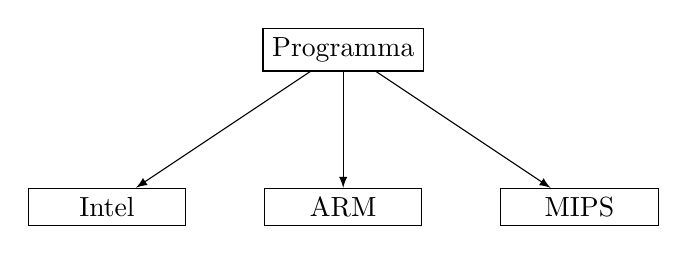
\begin{tikzpicture}[block/.style={draw,minimum width=2cm},
                        translate/.style={-latex}]
      \node[block] (source) at (0,2) {Programma};
      \node[block] (intel) at (-3,0) {Intel};
      \node[block] (arm) at (0,0) {ARM};
      \node[block] (mips) at (3,0) {MIPS};

      \draw[translate] (source) -- (intel);
      \draw[translate] (source) -- (arm);
      \draw[translate] (source) -- (mips);
    \end{tikzpicture}
  \end{center}
\end{frame}



%%% Local Variables:
%%% mode: latex
%%% TeX-master: "programming-languages"
%%% End:
